\documentclass[tikz,border=10pt]{standalone}
\usepackage{tikz}
\usepackage{fontawesome5}
\usetikzlibrary{arrows.meta,positioning,fit,backgrounds,calc,shadows,shapes.geometric}

\definecolor{civNavy}{RGB}{15, 34, 64}
\definecolor{civBlue}{RGB}{28, 80, 160}
\definecolor{civTeal}{RGB}{14, 130, 120}
\definecolor{civLightBlue}{RGB}{238, 245, 255}
\definecolor{civBorder}{RGB}{185, 210, 240}
\definecolor{civGold}{RGB}{217, 119, 6}
\definecolor{civGreen}{RGB}{22, 130, 80}
\definecolor{civDark}{RGB}{20, 28, 42}
\definecolor{cInput}{RGB}{240, 246, 255}
\definecolor{cStem}{RGB}{224, 242, 254}
\definecolor{cStage1}{RGB}{209, 250, 229}

\begin{document}
% Level-1 Data Flow Diagram (DFD) for CiviQ Platform
\begin{tikzpicture}[
    x=1cm, y=1cm,
    font=\sffamily,
    entity/.style={
        rectangle, draw=civNavy, line width=1.1pt, fill=white,
        rounded corners=3.5pt, minimum width=2.6cm, minimum height=1.15cm,
        align=center, font=\fontsize{8.5}{10.0}\selectfont\bfseries,
        drop shadow={shadow xshift=1.2pt, shadow yshift=-1.2pt, opacity=0.15}
    },
    process/.style={
        circle, draw=civNavy, line width=1.1pt, fill=cInput,
        minimum size=1.85cm, align=center,
        font=\fontsize{7.5}{8.8}\selectfont\bfseries,
        drop shadow={shadow xshift=1pt, shadow yshift=-1pt, opacity=0.12}
    },
    datastore/.style={
        rectangle, draw=civNavy!90, line width=0.95pt, fill=cStage1,
        minimum width=2.8cm, minimum height=0.85cm, align=center,
        font=\fontsize{7.5}{8.8}\selectfont\bfseries,
        drop shadow={shadow xshift=1pt, shadow yshift=-1pt, opacity=0.10}
    },
    dfdarr/.style={
        -{Stealth[scale=0.95]}, line width=0.95pt, draw=civNavy!90
    },
    flowlabel/.style={
        font=\fontsize{6.5}{7.5}\selectfont\bfseries, fill=white,
        draw=civNavy!25, line width=0.4pt, inner sep=2.0pt, rounded corners=2pt
    }
]

    % Row 1: Entities & Top Processes (y=7.2)
    \node (ecitizen) [entity] at (1.2, 7.2) {\faUser\ Citizen};
    \node (p1) [process] at (4.5, 7.2) {1.0\\Auth \&\\Profiles};
    \node (p5) [process] at (8.2, 7.2) {5.0\\Redressal\\\& Audit};
    \node (eadmin) [entity] at (11.8, 7.2) {\faUserShield\ Municipal\\Admin};

    % Row 2: Users Datastore (y=5.5)
    \node (d1) [datastore] at (4.5, 5.5) {D1: Users DB};

    % Row 3: Processing Core & Central Complaints Store (y=3.8)
    \node (p2) [process] at (1.2, 3.8) {2.0\\AI Vision\\Triage};
    \node (p3) [process] at (4.5, 3.8) {3.0\\GIS Ward\\Routing};
    \node (d2) [datastore, minimum width=2.9cm] at (8.2, 3.8) {D2: Complaints DB};
    \node (d6) [datastore] at (11.8, 3.8) {D6: Audit History Log};

    % Row 4: Spatial & Authority Datastores (y=2.2)
    \node (d3) [datastore] at (4.5, 2.2) {D3: GeoJSON Wards};
    \node (d4) [datastore] at (8.2, 2.2) {D4: Authorities DB};

    % Row 5: Civic Upvoting Process & Ledger (y=0.6)
    \node (p4) [process] at (1.2, 0.6) {4.0\\Civic\\Consensus};
    \node (d5) [datastore] at (4.5, 0.6) {D5: Upvotes DB};

    % Connections - Authentication Tier
    \draw [dfdarr] (ecitizen) -- node[above, flowlabel] {Credentials} (p1);
    \draw [dfdarr] (p1) -- node[right, flowlabel] {User Record} (d1);

    % Connections - Grievance Ingestion & AI Triage Tier
    \draw [dfdarr] (ecitizen) -- node[right, flowlabel] {Photo + GPS} (p2);
    \draw [dfdarr] (p2) -- node[above, flowlabel] {Defect Class} (p3);

    % Connections - Spatial Containment & Department Dispatch
    \draw [dfdarr] (d3) -- node[right, flowlabel] {Ward Polygons} (p3);
    \draw [dfdarr] (d4) -- node[right, flowlabel] {Dept Scopes} (d2);
    \draw [dfdarr] (p3) -- node[above, flowlabel] {Routed Issue} (d2);

    % Connections - Community Consensus Tier
    \draw [dfdarr] (p2) -- node[right, flowlabel] {Upvote Claim} (p4);
    \draw [dfdarr] (p4) -- node[above, flowlabel] {1-Upvote Unique} (d5);
    \draw [dfdarr] (p4.south) -- ++(0, -0.45) -| node[pos=0.3, above, flowlabel] {Priority Escalation ($\ge 3$)} (d2.south);

    % Connections - Municipal Redressal & Audit Trail Tier
    \draw [dfdarr] (d2) -- node[right, flowlabel] {Complaint State} (p5);
    \draw [dfdarr] (eadmin) -- node[above, flowlabel] {Status Update} (p5);
    \draw [dfdarr] (p5.south) to[out=-40, in=140] node[pos=0.45, above=2pt, flowlabel] {Audit Event Log} (d6.north west);

\end{tikzpicture}
\end{document}
